\section{Classical Robotics}

\epigraph{\textit{Know your enemy} [...]}{Sun Tzu}

\begin{tldr}
Robot learning is motivated by the need to (1) generalize across tasks and embodiments (2) reduce dependancy on human expertise (3) leverage historical trends on the production of data, all traditionally overlooked by legacy robotics techniques.
\end{tldr}

\subsection{Artificial Motion}
\label{sec:classical}

\begin{figure}
    \centering
    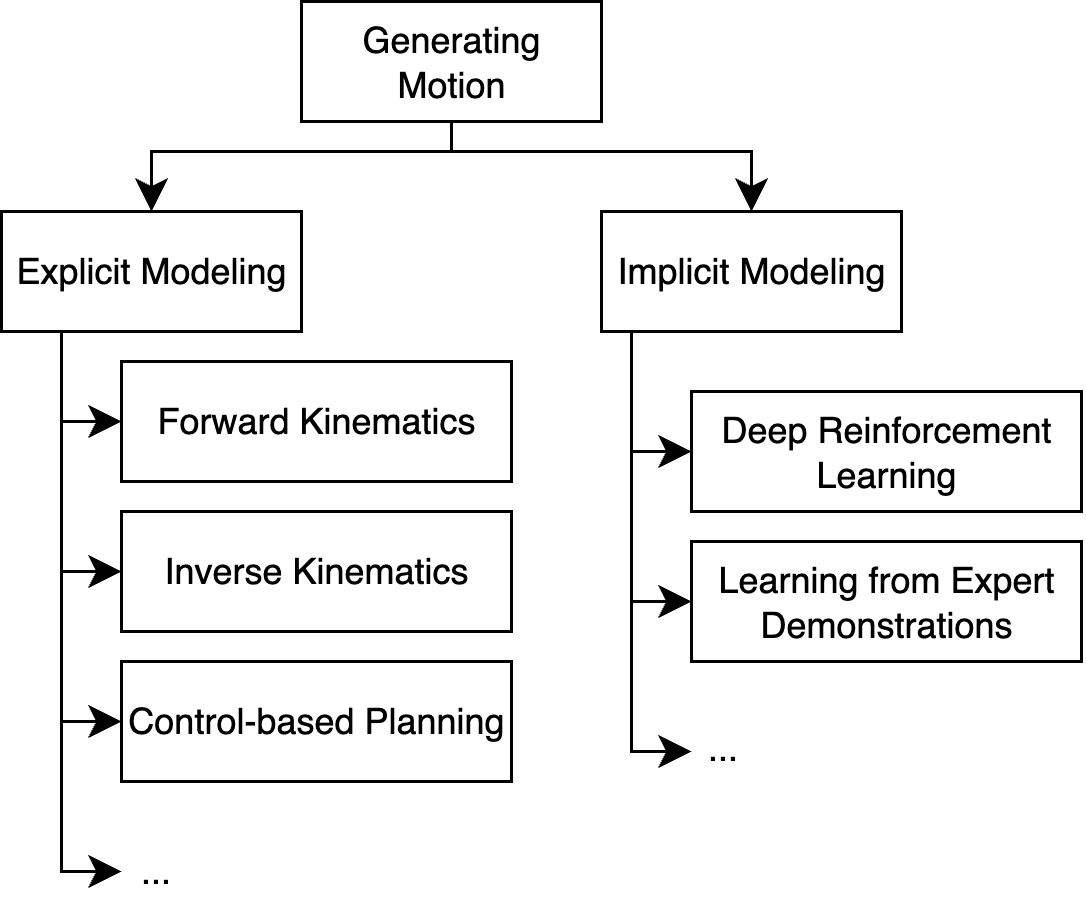
\includegraphics[width=0.5\linewidth]{figures/ch2/ch2-approaches.png}
    \caption{Overview of methods to generate motion (clearly non-exhausitve, see~\citet{bekrisStateRobotMotion2024}). The different methods can be grouped based on whether they explicitly (\emph{dynamics-based}) or implicitly (\emph{learning-based}) model robot-environment interactions.}
    \label{fig:generating-motion-atlas}
\end{figure}

Robotics is concerned with producing artificial motion in the physical world in a way that is useful, reliable and safe.
Thus robotics is at its very core an inherently multidisciplinar domain: producing motion requires interfacing various hardware and software componets, each at various levels.
Defining a concept of usefulness typically depends on a profound understanding of the applicative domain considered, whereas ensuring reliable and safe execution moreso relies on estimating the inhernet uncertainty in the robot's actions, guaranteeing adaptiveness of control while optimizing for performance, and more.
Knowledge of mechanical, electrical, and software engineering, as well as rigid-body mechanics and control theory have therefore been quintessential in robotics since the field first developed.
Lately, Machine Learning (ML) has proven useful in complementing said disciplines, making usage of the robotics data currently becoming more and more available.
As a direct consequence of its multi-disciplinar nature, robotics developed as a rather wide array of methods, all concerned with the main purpose of producing artificial motion in the physical world.

Methods to produce robotics motion range from traditional \emph{explicit} models---leveraging precise descriptions of the mechanics of robots' rigid bodies and their interactions with eventual obstancles in the robots environment---to fully \emph{learning-based} systems, offloading modelling the robot mechanics and rather treating motion as a statistical pattern to learn given multiple sensorimotor readings~\citep{bekrisStateRobotMotion2024}.
Between these two extrema, a variety of methods exists, with many borrowing traits from the opposite extremum to tackle specific challenges.
On the one hand, as learning-based systems can benefit from information relative to the physics of particularly static tasks, Temporal Difference (TD) methods have been complemented with Model-Predictive Control (MPC)~\citep{hansenTemporalDifferenceLearning2022}.
On the other hand, explicit models may be relying on assumptions proving overly simplicistic---or even unrealistic---in practice, as in the case of assuming perfect observability of a robot state using sensorimotor readings. In this context, feedback loops at the control level help mitigate the effects of poor state estimation, complementing the motion planning process with discrepancy-from-target information, similarily to how loss functions are used in statistical learning.
Figure~\ref{fig:generating-motion-atlas} graphically illustrates the most relevant techniques developed for general-purpose applications.
This categorization is far from being exhaustive, and we refer the interested reader to~\citet{bekrisStateRobotMotion2024} for a much more comprehensive overview of both general and application-specific methods for motion generation.
In this section, we aim at introducing the inherent benefit of learning-based approaches to robotics---the core focus on this tutorial---in the context of increasing availability of robot-data

\subsection{Different Types of Motion}

\begin{figure}
    \centering
    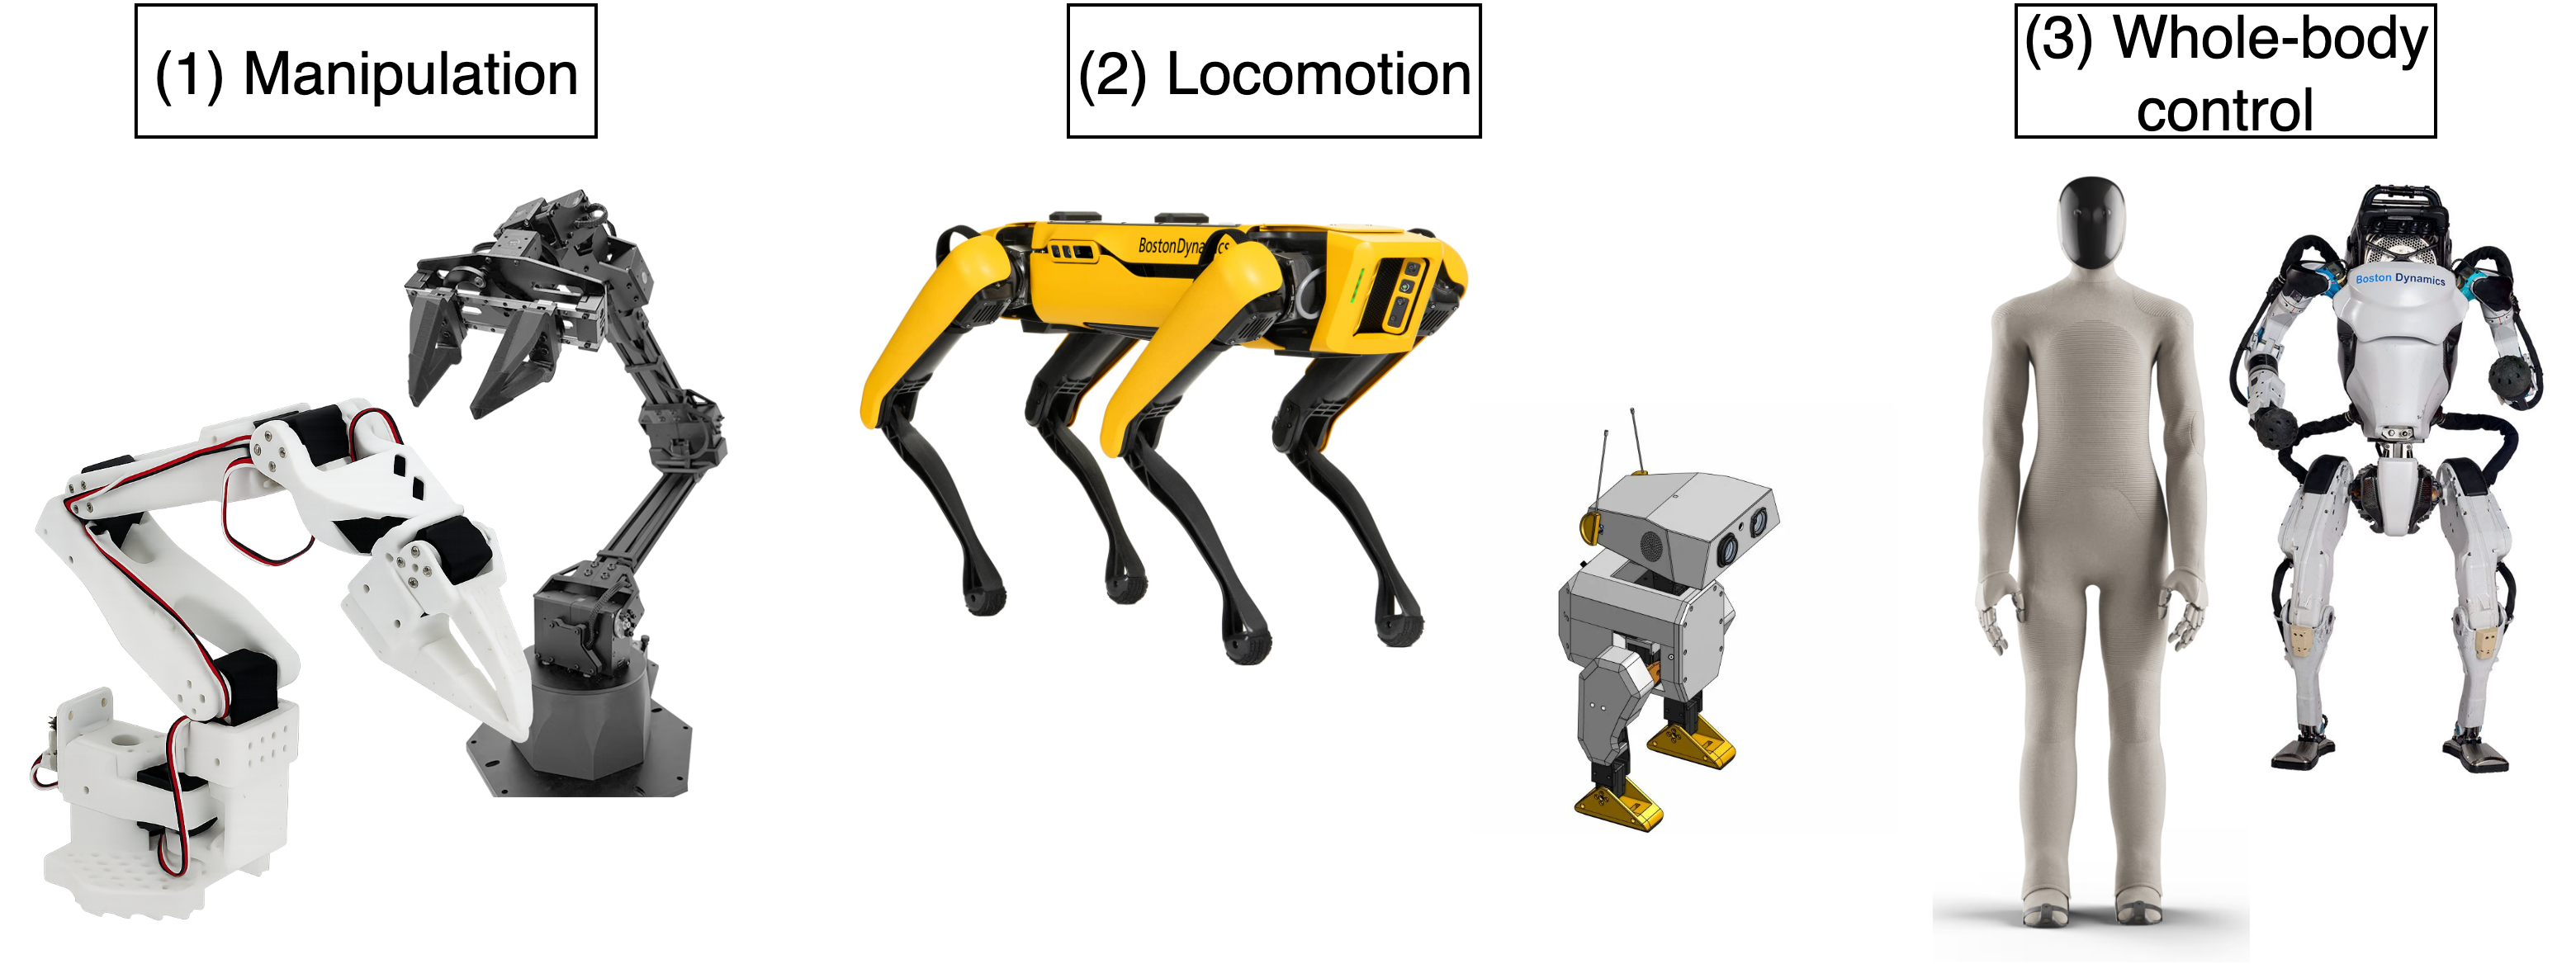
\includegraphics[width=0.7\linewidth]{figures/ch2/ch2-platforms.png}
    \caption{Different types of motions are achieved with potentially very different robotic platforms. From left to right, top to bottom: ViperX, SO-100, Boston Dynamics' Spot, Open-Duck, 1X's NEO, Boston Dynamics' Atlas. This list is (very) far from being exhaustive.}
    \label{fig:robotics-platforms-atlas}
\end{figure}

% Robotics atlas: moving through and modifying an environment (and combinations). That is, (1) locomotion (2) manipulation and (3) whole-body control
At its core, robotics deals with producing motion via actuating joints connecting nearly entirely-rigid links. 
A key distinction between focus areas in robotics is based on whether the generated motion modifies (1) the relative state of the robot with respect to its environment, (2) the absolute state of the environment or (3) both relative and absolute state (Figure~\ref{fig:robotics-platforms-atlas}).
For instance, (1) may consist in changes in the robot's physical location within its environment. 
Generally, modifications to a robot's location within its environment may be considered instances of the general \emph{locomotion} problem, further specified as \emph{wheeled} or \emph{legged} locomotion based on whenever a robot makes use of wheels or leg(s) to move in the environment.
Further, (2) are typically achieved \emph{through} the robot, i.e. generating motion to cause a perform an action inducing a desirable modification, effectively manipulating (\emph{manipulation}) the environment. 
Manipulation is a well studied problem class in robotics, nowadays solved in practice for static and repetitive manipulation tasks, typically performed in controlled and precisely studied scenarios for instance via industrial robots employed at various stages of manifacturing processes.
Lastly, an increased level of dynamism in the robot-environment interactions can be obtained combining (1) and (2), thus designing systems capable to move within \emph{and} interact with their environment, falling under the category of \emph{whole-body control}, and is characterized by a typically much larger set of control variables compared to either locomotion or manipulation alone.

% Focus on learning-based approaches and manipulation
The traditional body of work developed since the very inception of robotics is increasingly more complemented by learning-based approaches.
ML has indeed proven particularly transformative across the entire robotics stack, first empowering planning-based techniques with improved state estimation used for traditional planning~\citep{tangPerceptionNavigationAutonomous2023} and then end-to-end replacing controllers, from perception to action~\citep{koberReinforcementLearningRobotics}.
Work in producing robots capable of navigating a diverse set of terrains demonstrated the premise of both dynamics and learning-based approaches for locomotion~\citep{griffinWalkingStabilizationUsing2017,jiDribbleBotDynamicLegged2023,leeLearningQuadrupedalLocomotion2020,margolisRapidLocomotionReinforcement2022}, and recent works on whole-body control indicated the premise of learning-based approaches to generate rich motion in complex robot including humanoids~\citep{zhangWoCoCoLearningWholeBody2024,nvidiaGR00TN1Open2025}.
Manipulation has also been widely studied, particularly considering its aforementioned relevance for many impactful applications ranging from high-risk applications for humans~\citep{fujitaDevelopmentRobotsNuclear2020,alizadehComprehensiveSurveySpace2024,fujitaDevelopmentRobotsNuclear2020} to manifacturing~\citep{sannemanStateIndustrialRobotics2020}.
While explicit models relying on precise descriptions of the dynamics and knowledge of the robot-environment system have been the key milestones in the development of modern robotics, recent works leveraging learning-based techniques for manipulation proved particularly promising in surpassing scalability and practical applicability challenges~\citep{koberReinforcementLearningRobotics}.
Consequently, this work is primarily focused on the application of ML to robotics (\emph{robot learning}), and is particularly \emph{focused on manipulation}.

\subsection{Example: Planar Manipulation}

% Full physical description by means of forward kinmeatics to generate movement
Robot manipulators typically consist of a series of links and joints, all connected to an \emph{end-effector}.
In this example, we wish to provide a concrete example of a pick-and-place task, a relatively simple manipulation task whereby a robot reaches, grasps, moves and releases an object in space through a gripper end-effector.
Links and joints are considered responsible for generating motion, while the end effector is instead used to perform specific actions at the target location (e.g., grasping/releasing objects via closing/opening a gripper, using a specialized tool like a screwdriver or any measurement device).

Recently, the development of low-cost manipulators like the Aloha~\citep{zhaoLearningFineGrainedBimanual2023} Aloha-2~\citep{aldacoALOHA2Enhanced} and SO-100/SO-101~\citep{knightStandardOpenSO100} platforms significantly lowered the barrier to entry to robot learning research, considering their accessibility compared to more traditional platforms like the Franka Emika Panda arm (Figure~\ref{fig:robotic-platforms-costs},~\citep{knightStandardOpenSO100}). 
As a consequence, works on robot learning increasingly tackle the problem of learning to perform highly dexterous tasks using said low-end platforms: a long-standing challenge in manipulation.

\begin{figure}
    \centering
    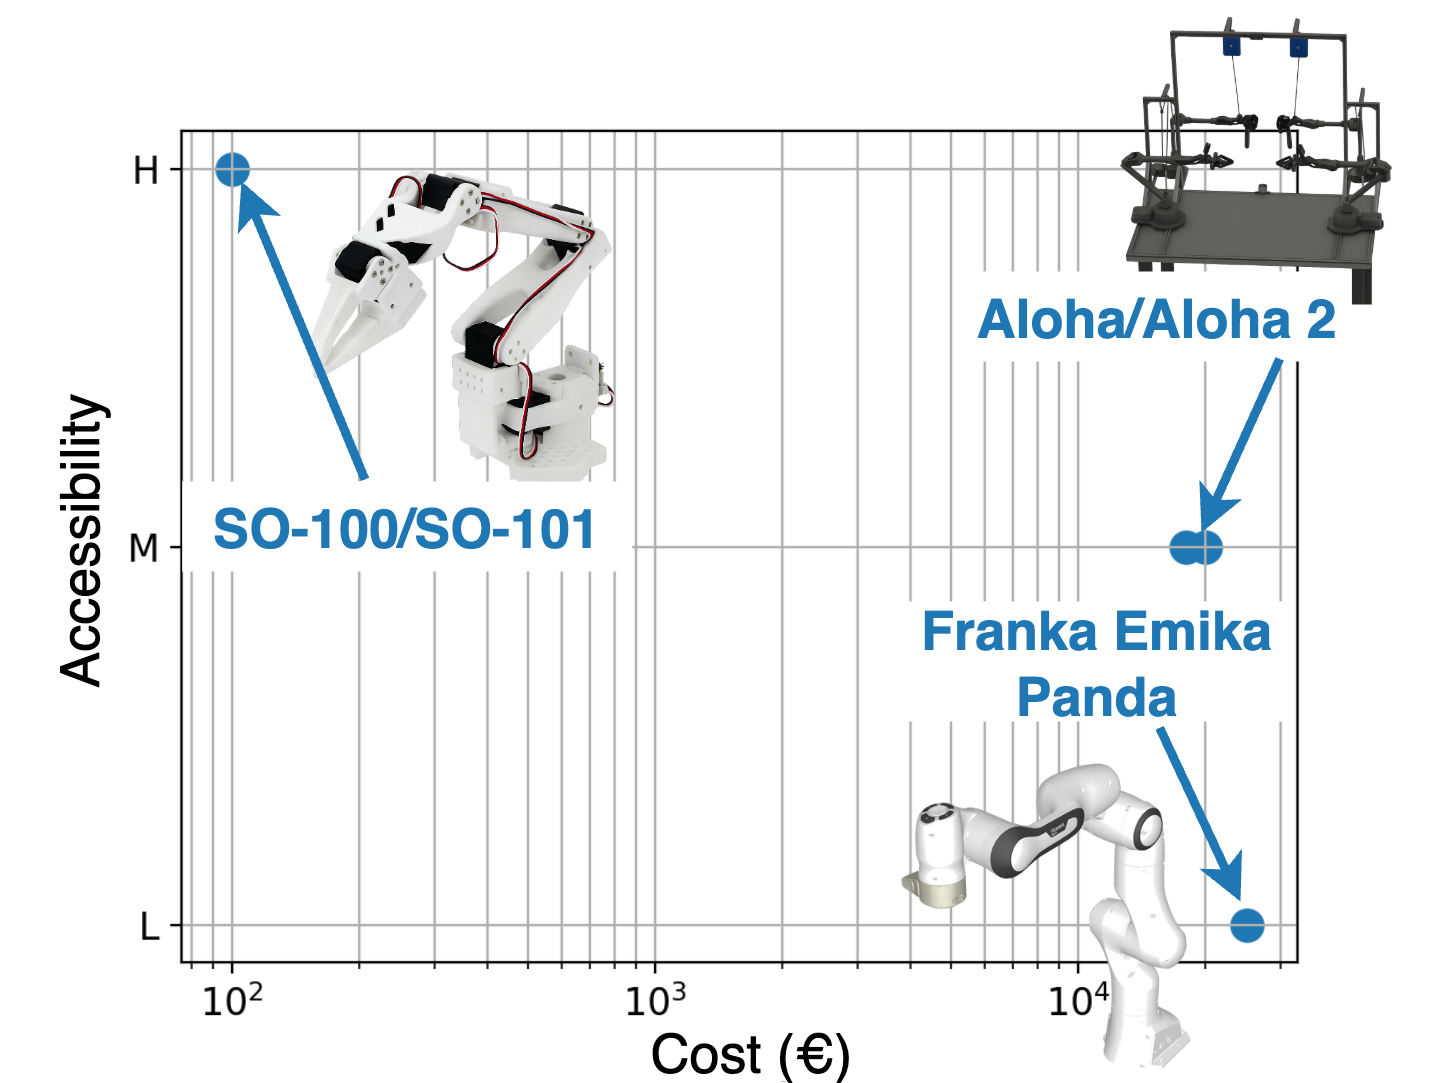
\includegraphics[width=0.4\linewidth]{figures/ch2/ch2-cost-accessibility.png}
    \caption{Cheaper, more accessible robots are starting to rival more traditional platforms like the Panda arm platforms in research and resource-constrained scenarios. The SO-100, in particular, has a cost in the 100s of Euros, and can be entirely 3D-printed, versus the industrially-manifactured Panda arm (tens of thousands of Euros).}
    \label{fig:robotic-platforms-costs}
\end{figure}

Deriving an intuition as per why learning-based approaches are gaining in popularity requires briefly analyzing traditional approaches for manipulation, leveraging forward/inverse kinematics and potentially control theory to account for disturbances and misestimations.
Traditionally, manipulation combines insights from fields including spatial algebra, optimization theory, control theory, and more. 
Providing a detailed overview of these fields fall (well) beyond the scope of this tutorial, hence we refer the reader to works including~\citet{sicilianoSpringerHandbookRobotics2016, lynchModernRoboticsMechanics2017, tedrakeRoboticManipulationPerception, tedrakeUnderactuatedRoboticsAlgorithms} for a more comprehensive description of these methods.
Here, we mostly wish to highlight the main reasons why the field of robotics is increasingly moving \emph{away} from these legacy methods.

\begin{figure}
    \centering
    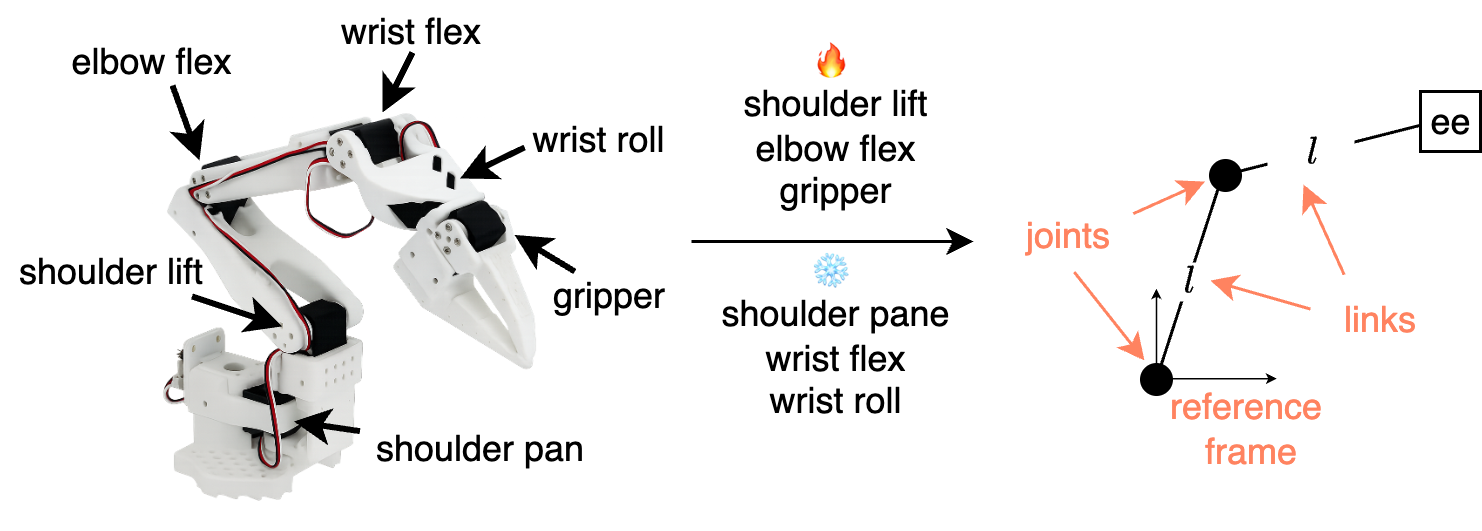
\includegraphics[width=0.7\linewidth]{figures/ch2/ch2-so100-to-planar-manipulator.png}
    \caption{The SO-100 arm is a 6-dof manipulator arm. Preventing some of its joints (shoulder pane, wrist flex and wrist roll) from actuating, it can be represented as a traditional 2-dof planar manipulator. The gripper joint in the end-effector is not considered towards the count of the degrees of freedom used to produce motion.}
    \label{fig:make-so100-planar-manipulator}
\end{figure}

Let us consider the (simple) case where the SO-100 is restrained from actuating (1) the shoulder pane and (2) the wrist flex and roll motors. 
This effectively reduces the degrees of freedom of the SO-100 from the original 5+1 (5 actuators + end effector) to 2+1 (shoulder lift, elbow flex + gripper), yielding the planar manipulator robot presented in Figure~\ref{fig:make-so100-planar-manipulator}, where spheres represent actuators yielding and lines links from the base of the stilifyied SO-100 to its end-effector (\emph{ee}, gripper).
Further, let us make the simplifying assumptions actuators can yield rotations in the links up to \( 2 \pi \) radians with respect to a given frame of reference.
In practice, this is seldom the case due to movement obstructions caused by the robot body. 
For instance, the shoulder lift cannot produce counter-clockwise movement due to the presence of the robot's base used to secure the SO-100 to its support and host the robot bus.
These simplifying assumptions leave us with the planar manipulator of Figure~\ref{fig:planar-manipulator-free}, free of moving its end-effector by controlling the angles \( \theta_1 \) and \( \theta_2 \), jointly referred to as \emph{robot's configuration} and indicated with \( q = [\theta_1, \theta_2 ] \in [0, 2\pi]^2 \).
In this tutorial, we do not cover spatial algebra and frames of reference, and we instead refer the interested reader to \cite[Chapter~2]{lynchModernRoboticsMechanics2017} and \cite[Chapter~3]{tedrakeRoboticManipulationPerception} for excellent explanations of mechanics and the theoretical foundations of producing motion.

\newcommand{\panelheight}{3.2cm}  % keeping the following manipulators aligned requires images to be same height

\begin{figure}
    \centering
    \begin{subfigure}[t]{0.32\linewidth}
        \centering
        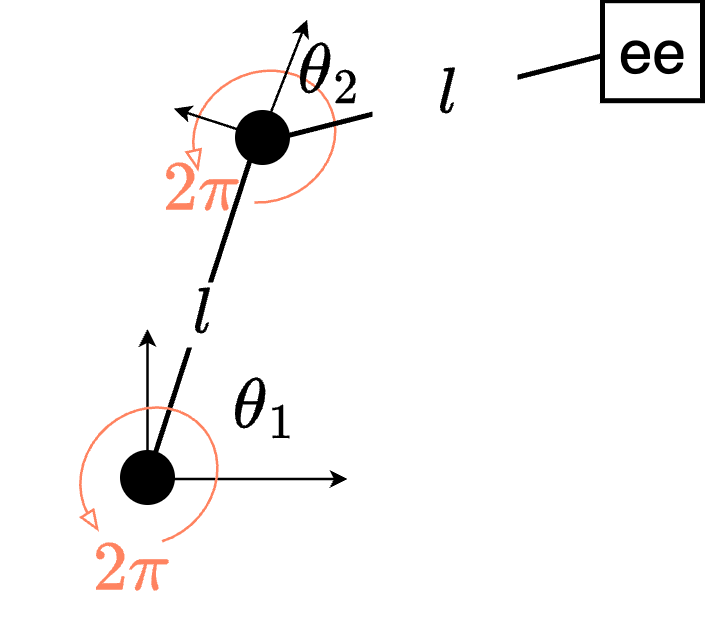
\includegraphics[width=\linewidth,height=\panelheight,keepaspectratio]{figures/ch2/ch2-planar-manipulator-free.png}
        \caption{Free of movement}
        \label{fig:planar-manipulation-simple}
    \end{subfigure}\hfill
    \begin{subfigure}[t]{0.32\linewidth}
        \centering
        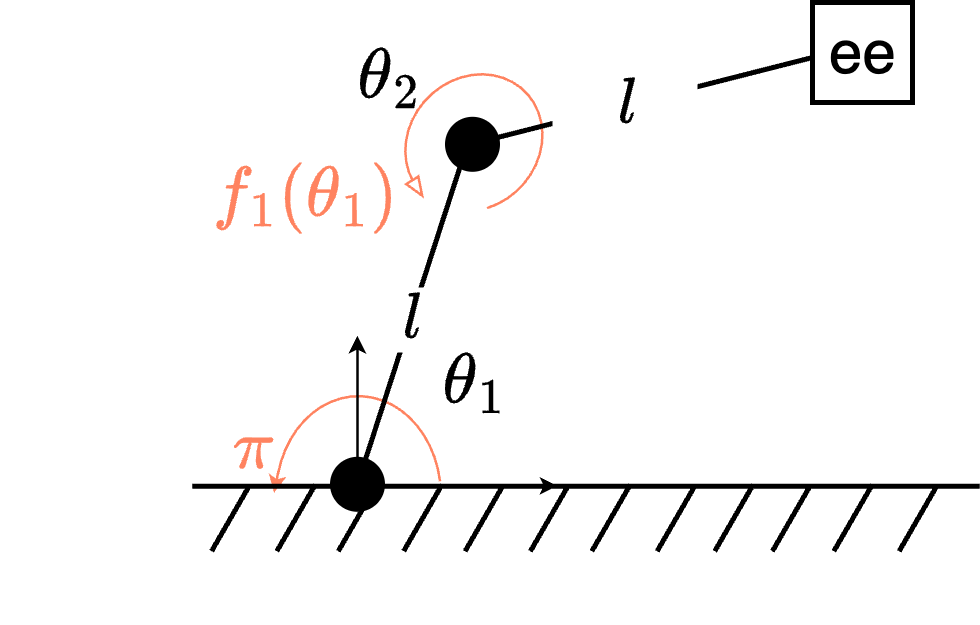
\includegraphics[width=\linewidth,height=\panelheight,keepaspectratio]{figures/ch2/ch2-planar-manipulator-floor.png}
        \caption{Constrained by the surface}
        \label{fig:planar-manipulator-floor}
    \end{subfigure}\hfill
    \begin{subfigure}[t]{0.32\linewidth}
        \centering
        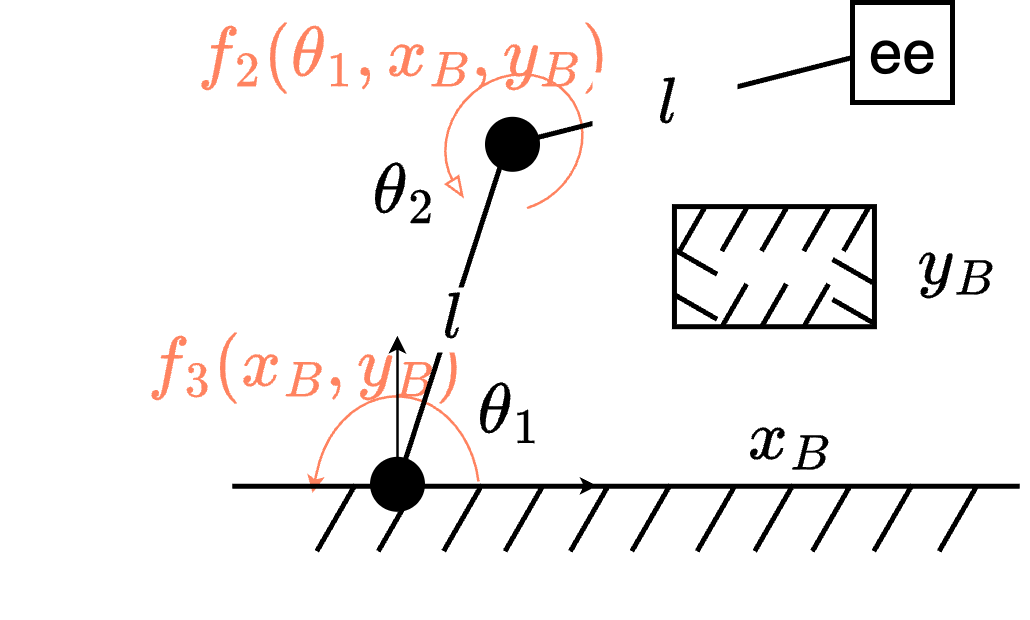
\includegraphics[width=\linewidth,height=\panelheight,keepaspectratio]{figures/ch2/ch2-planar-manipulator-floor-shelf.png}
        \caption{Constrained by surface and (fixed) obstacle}
        \label{fig:planar-manipulator-floor-shelf}
    \end{subfigure}
    \caption{Planar, 2-dof schematic representation of the SO-100 manipulator under diverse deployment settings. From left to right: completely free of moving ( \( \mathcal Q = [-\pihalf, +\pihalf]^2 \) ); constrained by the presence of the surface; constrained by the surface and presence of obstacles.}
\end{figure}

Considering the (toy) example presented in Figure~\ref{fig:planar-manipulation-simple}, then we can analytically write the end-effector's position \( p \in \mathbb R^2 \) as a function of the control applied, \( p = p(q), p: \mathcal Q \mapsto \mathbb R^2 \). 
In particular, we have:
\begin{equation*}
p(q) = 
\begin{pmatrix}
p_x(\theta_1, \theta_2) \\  
p_x(\theta_1, \theta_2)
\end{pmatrix}
=
\begin{pmatrix}
l_1 \cos(\theta_1) + l_2 \cos(\theta_1 + \theta_2) \\
l_1 \sin(\theta_1) + l_2 \sin(\theta_1 + \theta_2)
\end{pmatrix}
\end{equation*}
Deriving the end-effector's \emph{pose} \( p \in \mathcal{P} \subset \mathbb{R}^{\frac{n(n+1)}{2}} \) (position and orientation) starting from the configuration \( \q in \mathcal Q \subset \mathcal R^n \) of a \( n \)-joints robot is a problem referred to as \emph{forward kinematics} (FK), whereas identifying the configuration that corresponds to a given target pose is termed \emph{inverse kinematics} (IK).
In that, FK is used to map a robot configuration into end-effector position, whereas IK is used to derive what configuration(s) results in a given end-effector pose.
In the simplified case here considered, one can solve the problem of controlling the end-effector's location to reach a goal position \( p^* \) by solving analytically for \( q: p(q) = f_{\FK}(q) = p^*\).
However, in the general case, one might not be able to solve this problem analytically, and can typically resort to iterative optimization methods comparing candidate solutions based using a loss function (in the simplest case, \( \Vert p(q) - p^* \Vert_2^2 \) is a natural candidate), yielding:

\begin{align}
\min_{q \in \mathcal Q} \Vert p(q) - p^* \Vert_2^2
\label{eq:ik_problem}
\end{align}

Analytical solutions for FK are even less appealing when one considers the presence of obstacles in the robot's workspace, resulting in constraints on the possible values of \( q \in \mathcal Q \subset [-\pi, +\pi]^n \subset \mathbb R^n \) in the general case of \(n\)-links robots.
For instance, the robot in Figure~\ref{fig:planar-manipulator-floor} is (very naturally) obstacled by the presence of the surface upon which it rests: \( \theta_1 \) can now exclusively vary within \([-\pihalf,  \pihalf] \), while possible variations in \( \theta_2 \) depend on \( \theta_1 \) (when \( \theta_1 \to \pm \pihalf  \), further downwards movements are restricted).
Even for a simplified kinematic model such as the one considered here, solving~\ref{eq:ik_problem} is in general non-trivial, particularly considering an arbitrary \( \mathcal Q \) itself may change across problems.
Figure~\ref{fig:planar-manipulator-floor-shelf} provides another such example of how analytical solutions might fail to prove effective, even in our extremely simplified settings---if an obstacle was to be positioned in the robot environment, a new set of constraints based on the position of this new obstacle would emerge, potentially resulting in unfeasibility of the problem.

Further, IK---selecting the \( q \) solving \ref{eq:ik_problem}---only proves useful in determining information regarding to the robot's configuration in the goal configuration, and crucially does not provide information on the \emph{trajectory} to follow over time to reach a target pose.
\emph{Differential} inverse kinematics (diff-IK) complements IK by enabling trajectory tracking. 
Let \( J(q) \) denote the Jacobian matrix of (partial) derivatives of the FK-function \( f_\FK \mathcal Q \mapsto \mathcal P \), \( J(q) = \frac{\partial f_{FK}(q)}{\partial q } \), then one can apply the chain rule to any \( p(q) = f_{\FK}(q) \) deriving \( \dot p = J(q) \dot q \), finally relating variations in the robot configurations to variations in positions, thus providing a platform to for control.

Thus, given a desired end-effector velocity trajectory \( \targetvel \) indicating (1) which points in space to traverse and (2) how much time to spend in each region, diff-IK finds \( \dot q(t) \) by solving a \( \lambda \)-regularized version of \ref{eq:ik_problem}, solving for \emph{velocities} instead of \emph{positions},

\begin{align}
\dot q(t) = \arg\min_\nu \; \lVert J(q(t)) \nu - \targetvel (t) \rVert_2^2
\label{eq:reg_ik_velocity}
\end{align}

Unlike control in position, \( \dot q \) is much less dependent on the environment (typically, variations in velocity are constrained by physical limits on the actuators represented with box-like constraints in \ref{eq:reg_ik_velocity}.
Conveniently, \ref{eq:reg_ik_velocity} admits the closed-form solution, \( \dot q = J(q)^+ \targetvel \), where \( J^+(q) \) denotes the Moore-Penrose pseudo-inverse of \( J(q) \).
Finally, discrete-time trajectories can then obtained using forward integration,
\[
q_{t+1} = q_t + \Delta t\,\dot q_t
\]
Following trajectories with diff-IK is a valid option in well-controlled and static environments like manipulators in industrial applications, and relies on the ability to define a set of target velocities to track \( [\targetpos_0, \targetpos_1, \dots, \targetpos_k ] \)---a task largely carried out by human experts and prone to errors.
Furthermore, diff-IK relies on the ability to (1) access \( J(q) \, \forall q \in \mathcal Q \) and (2) compute its pseudo-inverse at every iteration of a given control cycle---an assumption complicated to guarantee in highly dynamical settings or for complex instances of FK (nonlinear dynamics).

\subsubsection{Adding Feedback Loops}
While effective when a goal has been well specified, the performance of diff-IK can degrade significantly in the presence of modeling/tracking errors or in the presence of non-modeled dynamics in the environment.

\begin{wrapfigure}[16]{r}{0.3\textwidth}
    \vspace{-\intextsep}
    \centering
    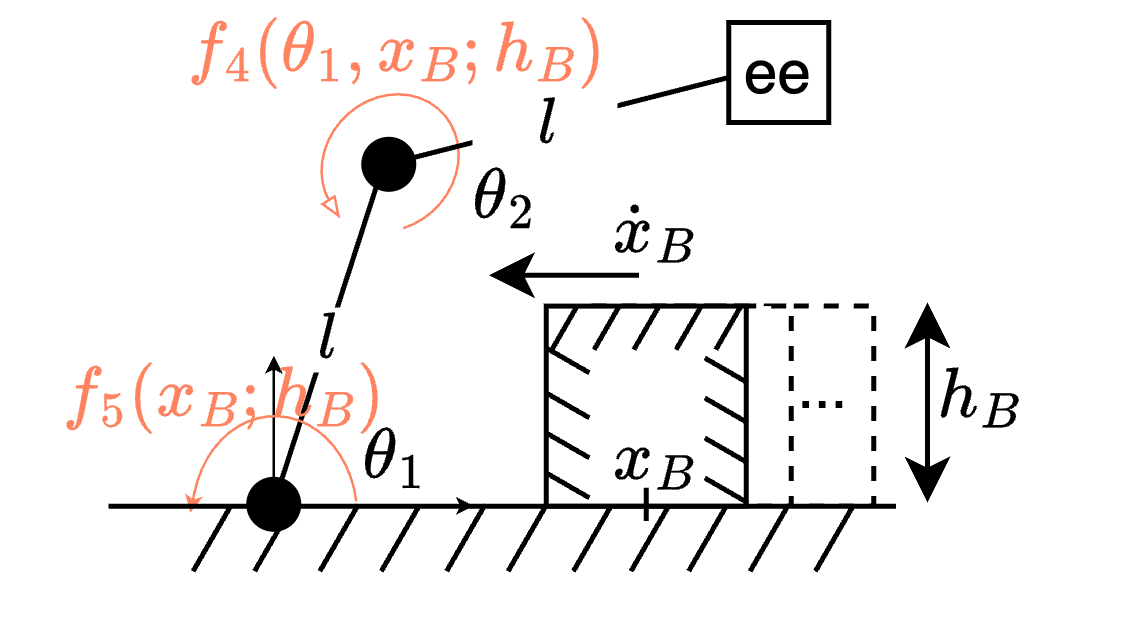
\includegraphics[width=\linewidth]{figures/ch2/ch2-planar-manipulator-floor-box.png}
    \caption{Planar manipulator robot in the presence of a moving obstacle. The position and velocity of the obstance influence the range of possible controls that can be safely applied on the robot, and thus must be considered for control.}
    \label{fig:planar-manipulator-box-velocity}
\end{wrapfigure}

One such case is presented in Figure~\ref{fig:planar-manipulator-box-velocity}, where another rigid body is moving in the environment along the horizontal axis, with velocity \( \dot x_B \).
Accounting analytically for the presence of this disturbance---for instance, to prevent \( l_1 \) from ever colliding with the object---requires access to \( \dot x_B \) and of a reference position \( x_{B,0} \) for the object \( B \), to derive the equation characterizing its motion.
For less predictable disturbances (e.g., \( \dot x_B \leftarrow x_B + \eps, \eps \sim N(0,1) \) one could attain similar results by adding a condition on the distance between the midpoint of \( l_1 \) and \( x_B \), enforced through a feedback loop on the position of the robot and object at each control cycle.

To mitigate the effect of modeling errors, sensing noise and other disturbances, classical pipelines augment diff-IK with feedback control on the measured error between the target position and the one measured, \( \Delta p = \targetpos - p(q) \), hereby modifying the control applied to \( \dot q = J(q)^+ (\targetvel + \lambda \Delta p \), with \( \lambda \) defined as the gain.
More advanced techniques for control consisting in feedback linearization, PID control, or LQR/MPC can also be employed to stabilize tracking and reject moderate perturbations (\cite[Chapter~8]{sicilianoSpringerHandbookRobotics2016}, or \cite[Chapter~8]{tedrakeRoboticManipulationPerception} for a simplified example in the case of a point-mass system).
Nonetheless, tuning gains remains laborious and system-specific: In manipulation, intermittent contacts induce hybrid dynamics (mode switches) and discontinuities in the effective Jacobian, challenging stability guarantees and often necessitating conservative gains and substantial hand-tuning.

We point the interested reader to \cite[Chapter~2,7,8]{sicilianoSpringerHandbookRobotics2016}, \cite[Chapter~6,11]{lynchModernRoboticsMechanics2017}, and \cite[Chapter~3,8]{tedrakeRoboticManipulationPerception} for extended coverage of FK, IK and diff-IK and control for (diff-)IK.

\subsection{Limitations of Classical Robotics}
Depiste the last 60+ years of robotics research, autonomous robots are still largely incapable of performing tasks at human-level performance in the physical world across (1) robot embodiments (different manipulators, different locomotion platforms, etc.) and (2) tasks (tying shoe-laces, manipulating a diverse set of objects).
While essential in the early development of robotics, the aforementioned methods require significant human expertise to be used in practice, and are typically specific to a particular applicative problem. 

\begin{figure}
    \centering
    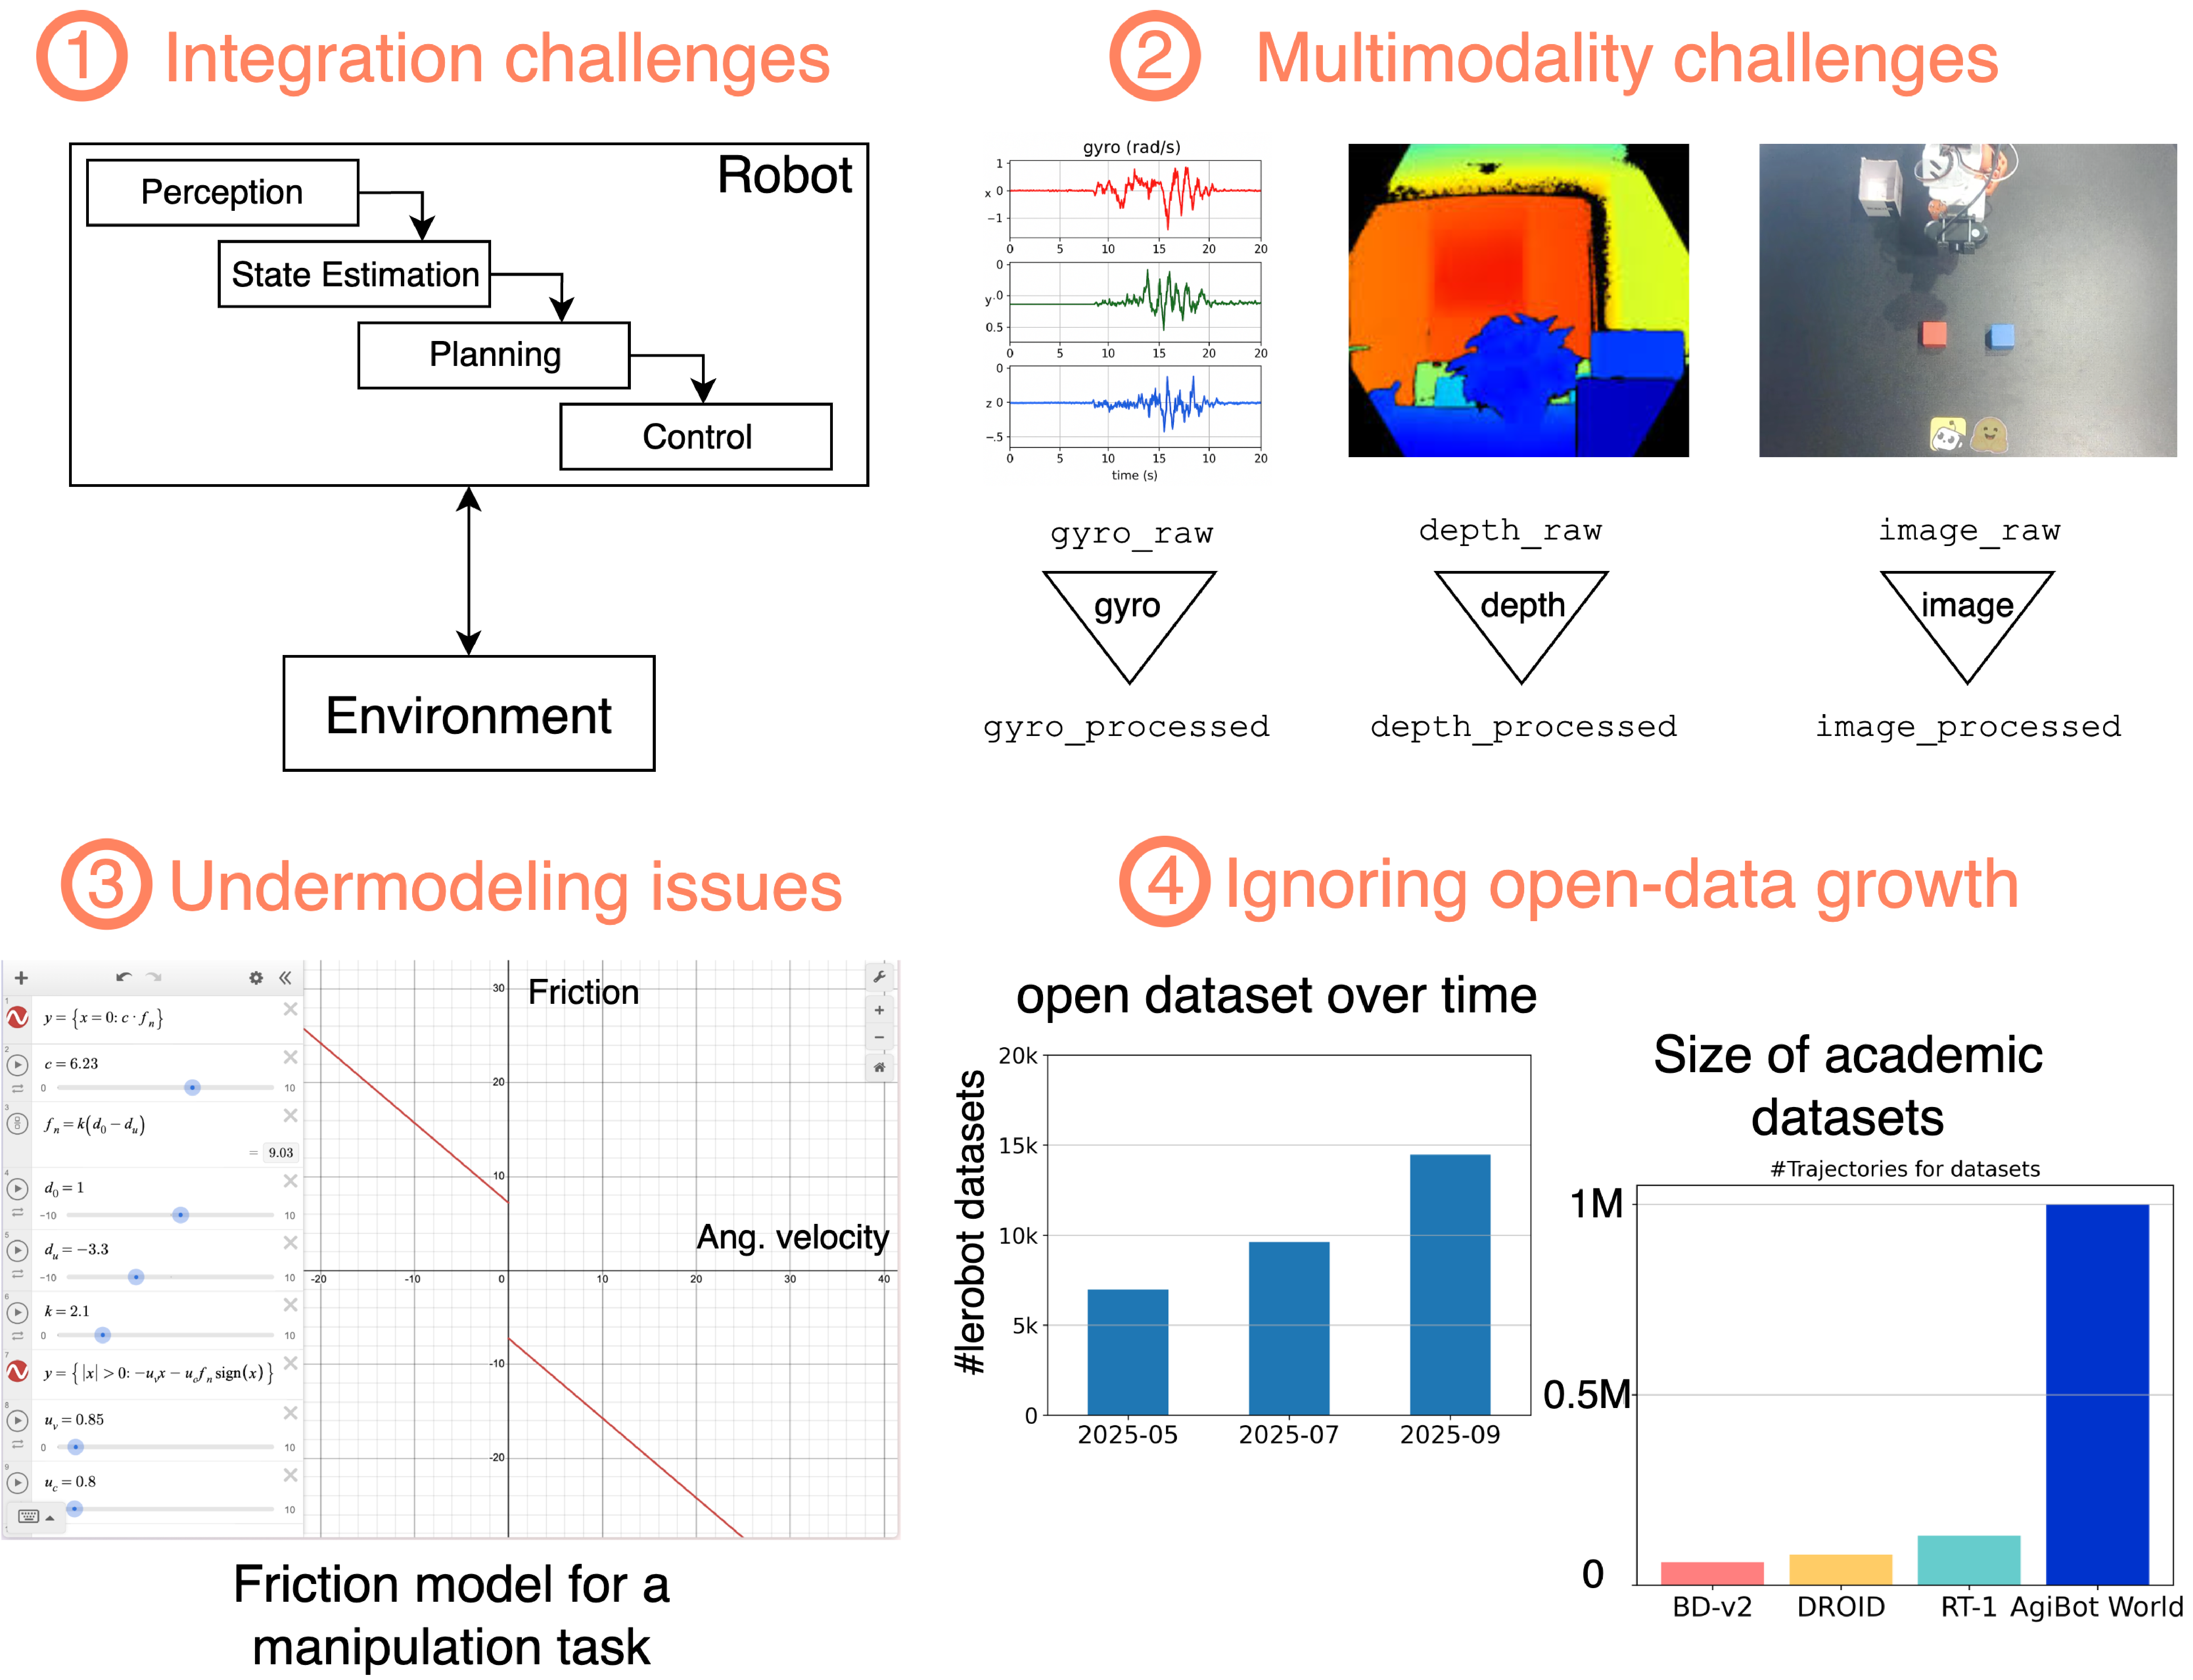
\includegraphics[width=0.9\linewidth]{figures/ch2/ch2-classical-limitations.png}
    \caption{Dynamics-based approaches to robotics suffer from several limitations: (1) orchestrating multiple components poses integration challenges; (2) the need to develop custom processing pipelines for the sensing modalities and tasks considered hinders scalability; (3) simplified analytical models of physical phenomena (here friction at the gripper; credits to~\citet{antonovaReinforcementLearningPivoting2017}) limit real-world performance. Lastly, (4) dynamics-based methods overlook current trends in the growth of robotics data.}
    \label{fig:classical-limitations}
\end{figure}

Robotics pipelines have been \highlight{developed sequentially, hand-engineering the different block architectures} for specific purposes. 
Sensing, state estimation, mapping, planning, (diff-)IK, and low-level control have been traditionally developed as distinct modules with fixed interfaces.
Pipelining these highly specific modules is a error-prone, and brittleness emerges whenever shifts with respect to a considered pipeline incur (e.g., changes in lighting for sensing, occlusion/failure of sensors).
Adapting such a stack to new tasks or embodiments often entails re-specifying objectives, constraints, and heuristics at multiple stages, incurring significant engineering overhead.

Classical planners operate on compact, assumed-sufficient state representations; extending them to reason directly over raw, heterogeneous and noisy data streams is non-trivial.
This results in a \highlight{limited scalability to multimodal data and multitask settings}, as incorporating high-dimensional perceptual inputs (RGB, depth, tactile, audio) traditionally required extensive engineering efforts to extract meaningful efforts for control. 
Moreover, the large number of tasks, coupled with the adoption of \emph{per-task} planners, goal parameterizations, and safety constraints, results in an explosion in design and validation effort, with little opportunity to share experience across tasks.

Further, even setting aside integration and scalability challenges, developing accurate modeling of contact, friction, and compliance for complicated remains difficult.
Rigid-body approximations are often insufficient in the presence of deformable objects, and \highlight{relying on approximated models hinders real-world applicability}.
In the case of complex and/or non-linear dynamics, even moderate mismatches in contact parameters, unmodeled flexibilities, or grasp-induced couplings can qualitatively affect the observed dynamics, degrading the reliability of  the model obtained.
Even a perfect model of reality would need to relax the stationarity assumptions that are typically made in control. Explicitly modeling the effects of payload changes, tool substitutions, temperature-dependent friction, and component-aging on the resulting dynamics is, in most cases, simply unfeasible.

Lastly, dynamics-based methods (naturally) overlook the rather recent phenomenon of the \highlight{explosion of openly-available robotics data}, following a similar pattern to the explosion of image and text data.
The curation of academic datasets by large centralized groups of human experts in robotics~\citep{OpenXEmbodimentRobotic,DROIDLargeScaleIntheWild,agibot-world-contributorsAgiBotWorldColosseo2025} is now increasingly complemented by a \highlight{growing number of robotics datasets contributed in a decentralized fashion} by individuals with varied expertises.
If not tangentially, dynamics-based approaches are not posed to maximally benefit from this new trend, holding the premise of allowing generalization in the space of tasks and embodiments, like data was the cornerstone for advancements in vision~\citep{alayracFlamingoVisualLanguage2022} and natural-language understanding~\citep{openaiGPT4TechnicalReport2024}.

Taken together, these limitations (Figure~\ref{fig:classical-limitations}) motivate the exploration of learning-based approaches that can (1) integrate perception and control more tightly, (2) adapt across tasks and embodiments with reduced expert intervention and (3) scale gracefully in performance as more robotics data becomes available.